\documentclass[../main.tex]{subfiles}

\begin{document}

\section{Results}


\subsection{Fluorescent Proteins}

With kind support from other sources (see section~\ref{sec:plaspri:plas}) we built up a library of many fluorescent protein-chemotaxis protein fusions. However, it was still necessary to exchange many of these. Many fluorescent proteins (e.g. CFP, YFP, BFP) are all derivatives of GFP through only a few amino acid substitutions~\citep{tsien98}. In most modernly used GFP derivatives, these all lie between amino acid 64 and amino acid 206, inclusive. Therefore, through careful design of PCR primers Gibson assembly can be used to exchange one GFP derivative for another with the same set of primers (see section~\ref{sec:plaspri:pri}).

Primarily EYFP was used for the proteins being imaged. However, a monomeric form was required for anisotropy~\citep{vaknin07}, requiring the mutation A206K. Another EYFP varaent, known as Venus, was described as being a better FRET receiver~\citep{nagai02} as well as a generally improved fluorophore, and therefore ideal for our anisotropy experiments. However, only the monomeric EYFP variant was available to us, and we have not yet had time to perform the five amino acid substitutions required for Venus.

Site directed mutagenisis was initially to be used to create the mutations from EYFP to Venus, but this was not followed through due to cost and also after receiving what was described as Venus, but which turned out to be the EYFP with the A206K mutation.

Primers for standard cloning with multiple restriction sites were designed (see section~\ref{sec:plaspri}); however, after repeated attempts we failed to obtain a final construct, and after several weeks this assembly method was abandoned.

Gibson assembly worked on the first time, and was used with a perfect success rate for all subsequent exchanges. Plasmids were split in to two to ensure that PCR would be able to run their entire length. 

\begin{figure}
\begin{center}
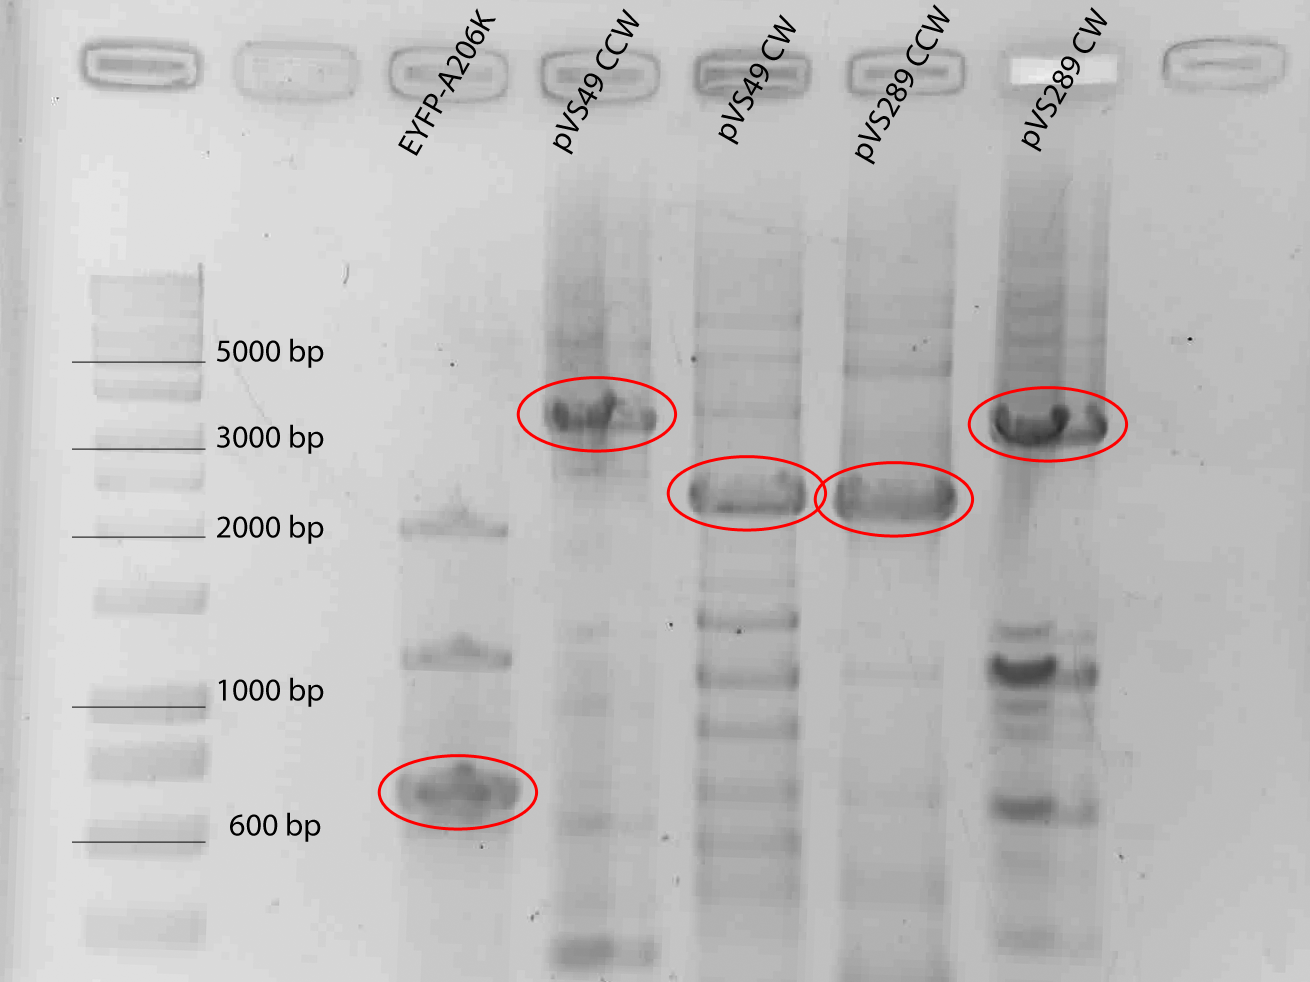
\includegraphics[width=\textwidth]{\docroot results/figs/gibsonpcr.png}
\caption[PCR results for Gibson Assembly]{PCR to create overlaps for Gibson Assembly. Desired bands circled in red. Whilst each of the five PCR reactions had a lot of misprimes and over-extensions, the desired bands were strong enough to be easily visible, and after gel extraction specific enough to perform Gibson assembly successfully.}
\end{center}
\end{figure}
\newpage
\subsection{Inducer Calibration}

Most fusion proteins were available, or could easily be made available, in both the pBAD33 or pTRC99a plasmid, induced by arabinose or IPTG respectively. As in some experiments we planned to induce two proteins using both, it was important to be able to balance the production of each, by performing titrating the inducer concentration. The expression of \textsl{CheZ-eYFP} was monitored in two strains, KL1001 and KL10019, induced by Arabinose and IPTG respectively (for details, see section~\ref{sec:plaspri}).

Images are shown of each of four different concentrations of inducer \SI{3.5}{\hour} after induction in each strain.

\begin{figure}
\begin{center}
\subfloat[0.001\% Arabinose]{
	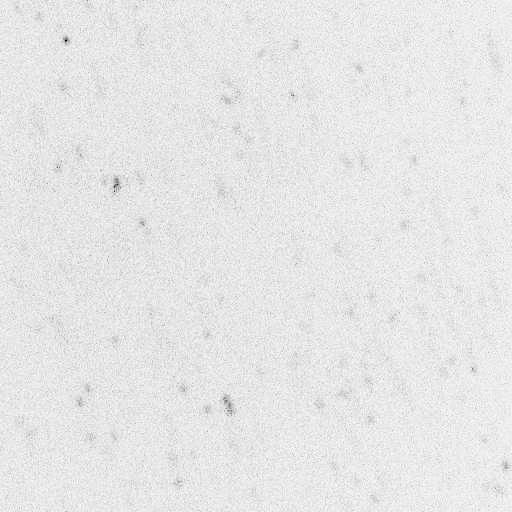
\includegraphics[width=.45\linewidth]{\docroot results/figs/A1-yfp.jpg}
}
\subfloat[0.005\% Arabinose]{
	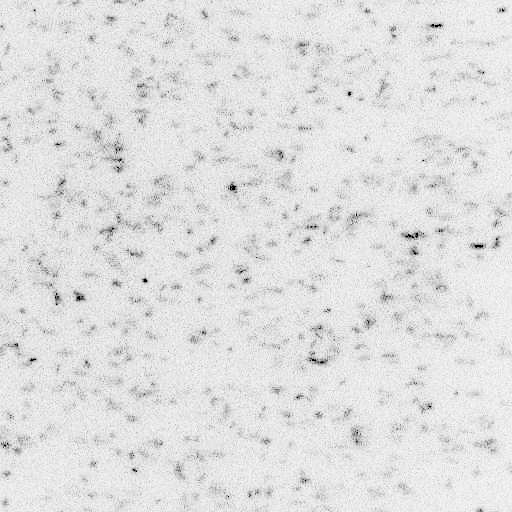
\includegraphics[width=.45\linewidth]{\docroot results/figs/A2-yfp.jpg}
}\\
\subfloat[0.01\% Arabinose]{
	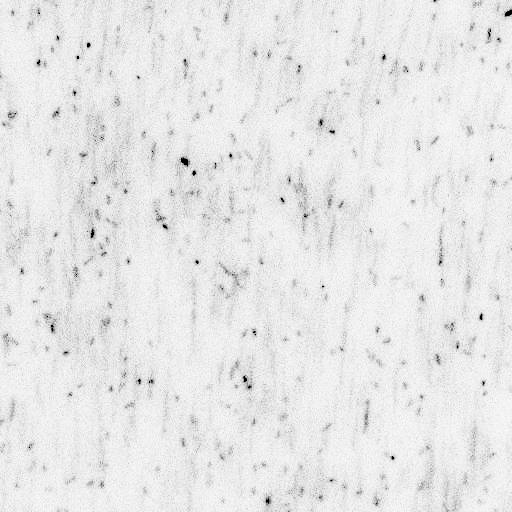
\includegraphics[width=.45\linewidth]{\docroot results/figs/A3-yfp.jpg}
}
\subfloat[0.05\% Arabinose]{
	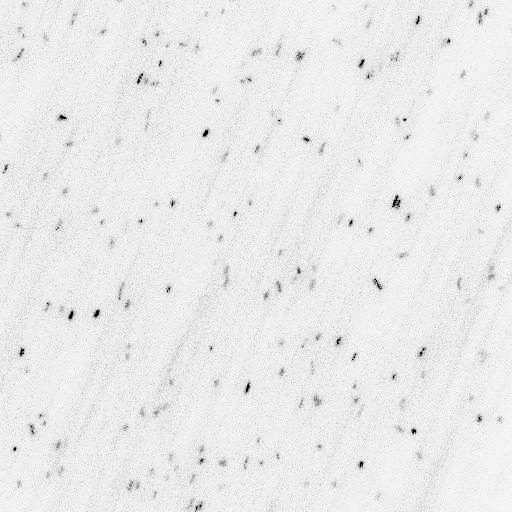
\includegraphics[width=.45\linewidth]{\docroot results/figs/A4-yfp.jpg}
}
\caption[Arabinose inducer titration]{Arabinose inducing \textsl{CheZ-eYFP} expression in KL1001. Colours inverted to improve printed contrast.}
\end{center}
\end{figure}

\begin{figure}
\begin{center}
\subfloat[\SI{5}{\micro\Molar} IPTG]{
	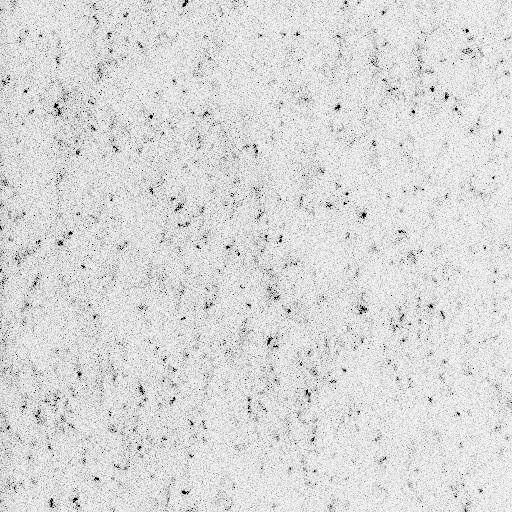
\includegraphics[width=.45\linewidth]{\docroot results/figs/S5-yfp.jpg}
}
\subfloat[\SI{10}{\micro\Molar} IPTG]{
	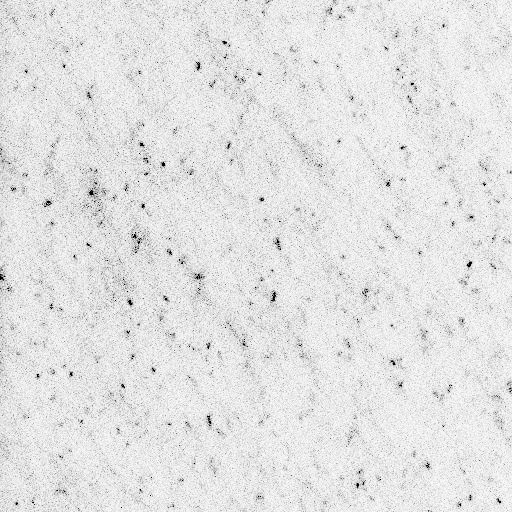
\includegraphics[width=.45\linewidth]{\docroot results/figs/S6-yfp.jpg}
}\\
\subfloat[\SI{20}{\micro\Molar} IPTG]{
	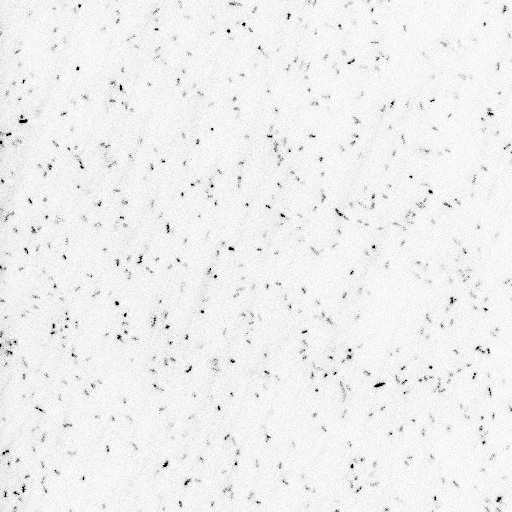
\includegraphics[width=.45\linewidth]{\docroot results/figs/S7-yfp.jpg}
}
\subfloat[\SI{40}{\micro\Molar} IPTG]{
	
\includegraphics[width=.45\linewidth]{\docroot results/figs/S8-yfp.jpg}
}
\caption[IPTG inducer titration]{IPTG inducing \textsl{CheZ-eYFP} expression in KL1019. Colours inverted to improve printed contrast.}
\end{center}
\end{figure}




\begin{comment}
\paragraph{Inducement time.} Generally it is recommended to induce some time after inoculating fresh media with overnight cultures; however this is not necessary if the proteins being induced are not toxic. Two parallel growths were done, OD measurements taken every two hours, and images recorded 4 hours after induction and four hours after inoculation.
\begin{center}
\begin{tabular}{ccc}
t=0	&	Inoculate	&	Inoculate \& Induce\\
2	&	Induce	&\\
4	&	Image	&	Image\\
6	&	Image	&
\end{tabular}
\end{center}

\paragraph{Inducer Titre} A logarithmic course of inducer concentrations was checked for expression of the same fusion protein under different promoters.

\begin{center}
\begin{tabular}{cc}
\textbf{Arabinose}	&	\textbf{IPTG} 	\\
0.001\%	&	\SI{1}{\micro\Molar}\\
0.003\%	&	\SI{3}{\micro\Molar}\\
0.01\%	&	\SI{10}{\micro\Molar}\\
0.03\%	&	\SI{30}{\micro\Molar}\\
0.1\%	&	\SI{100}{\micro\Molar}\\

\end{tabular}
\end{center}

\paragraph{Time Course}	A selection of inducer concentration from the inducer titre were re-run with samples being removed and imaged at \SI{2}{\hour}, \SI{3}{\hour} and \SI{4}{\hour} to find optimal expression.
 \end{comment}

\newpage
\subsection{Cluster Sizing using Image Processing}

The following section contains results from image processing based techniques as described in section~\ref{sec:methods:imageprocessing}.

\subsubsection{Epifluorescence Microscopy}
\label{sec:results:cs:epi}

These experiments were performed on a Nikon microscope on loan from the manufacturer. One image was taken each from a slide of cells prepared with and without cobalt.

\begin{figure}[h!]
\begin{center}
\subfloat[No cobalt, \(n=18, \mu=0.144, \sigma=0.070\)]{
	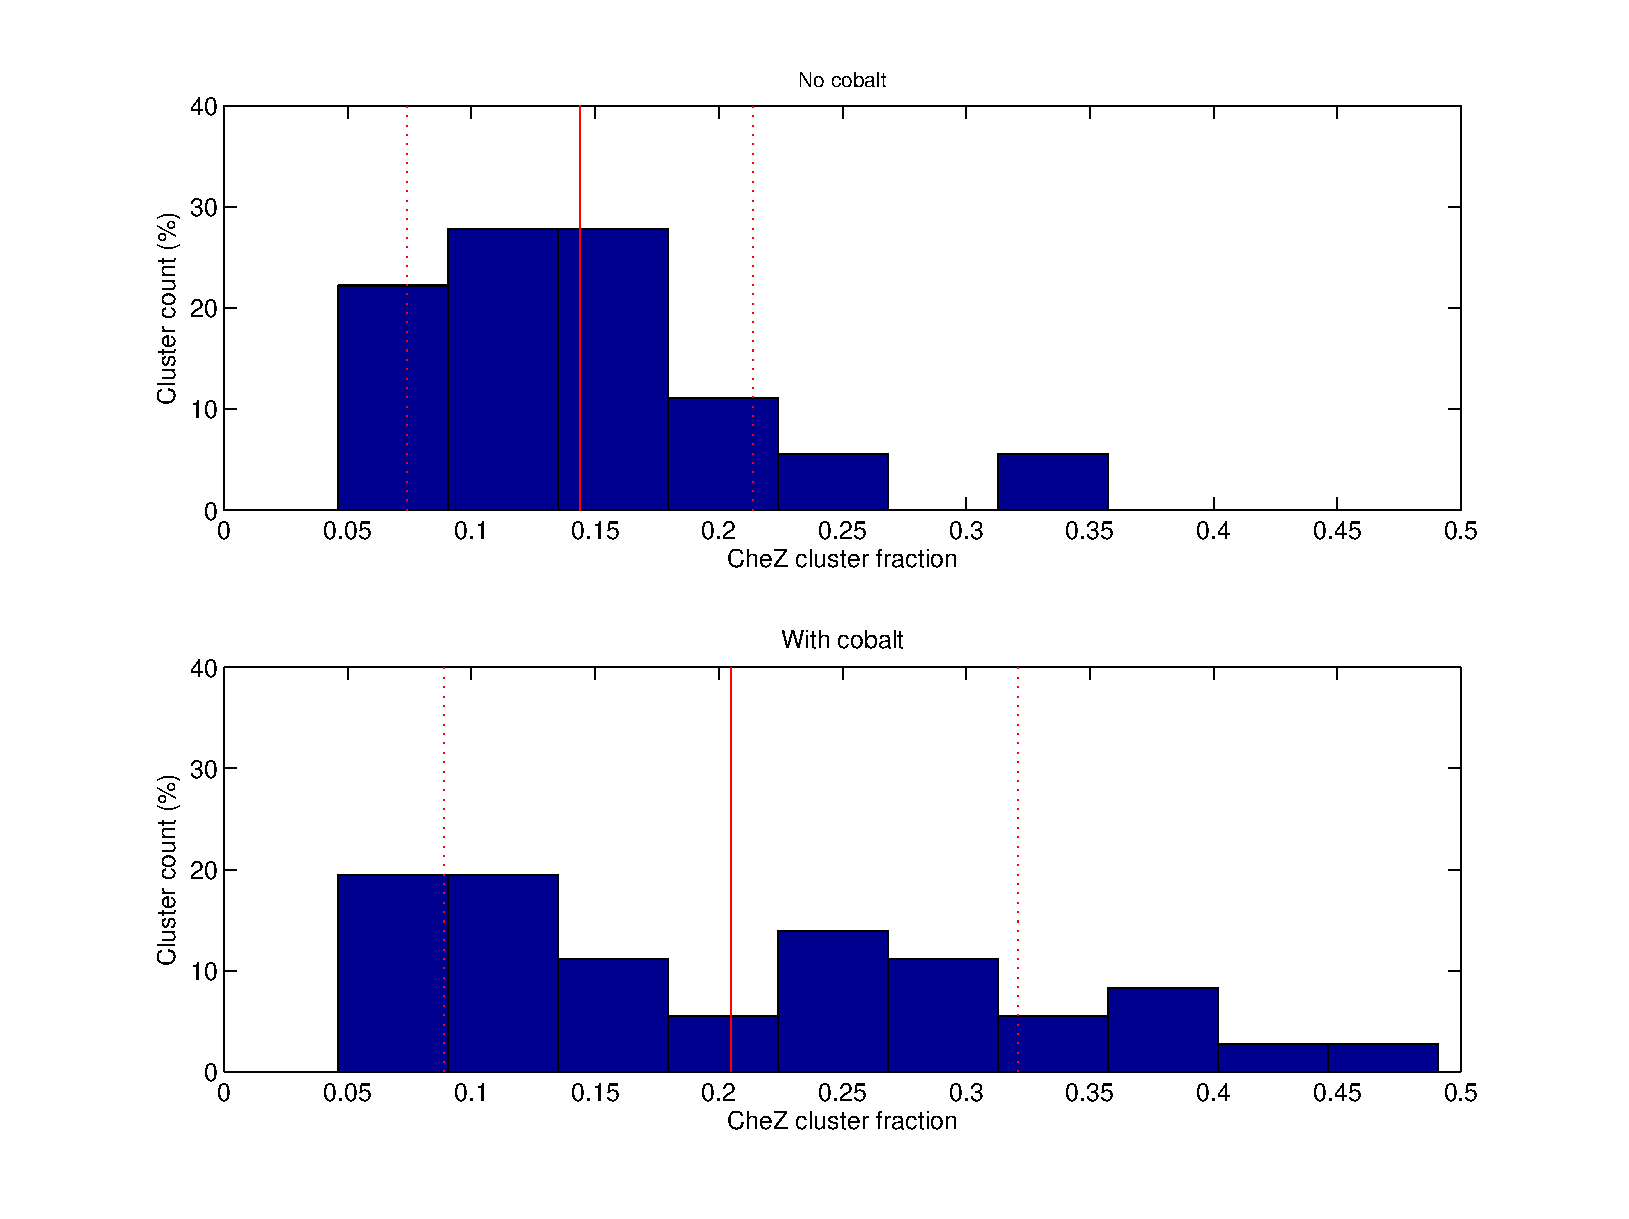
\includegraphics[scale=0.65, trim=0 300 0 40, clip=true]{\docroot results/figs/nikonb.eps}
	\label{fig:results:nikon:nocobalt}
}\\
\subfloat[With cobalt, \(n=36, \mu=0.205, \sigma=0.116\)]{
	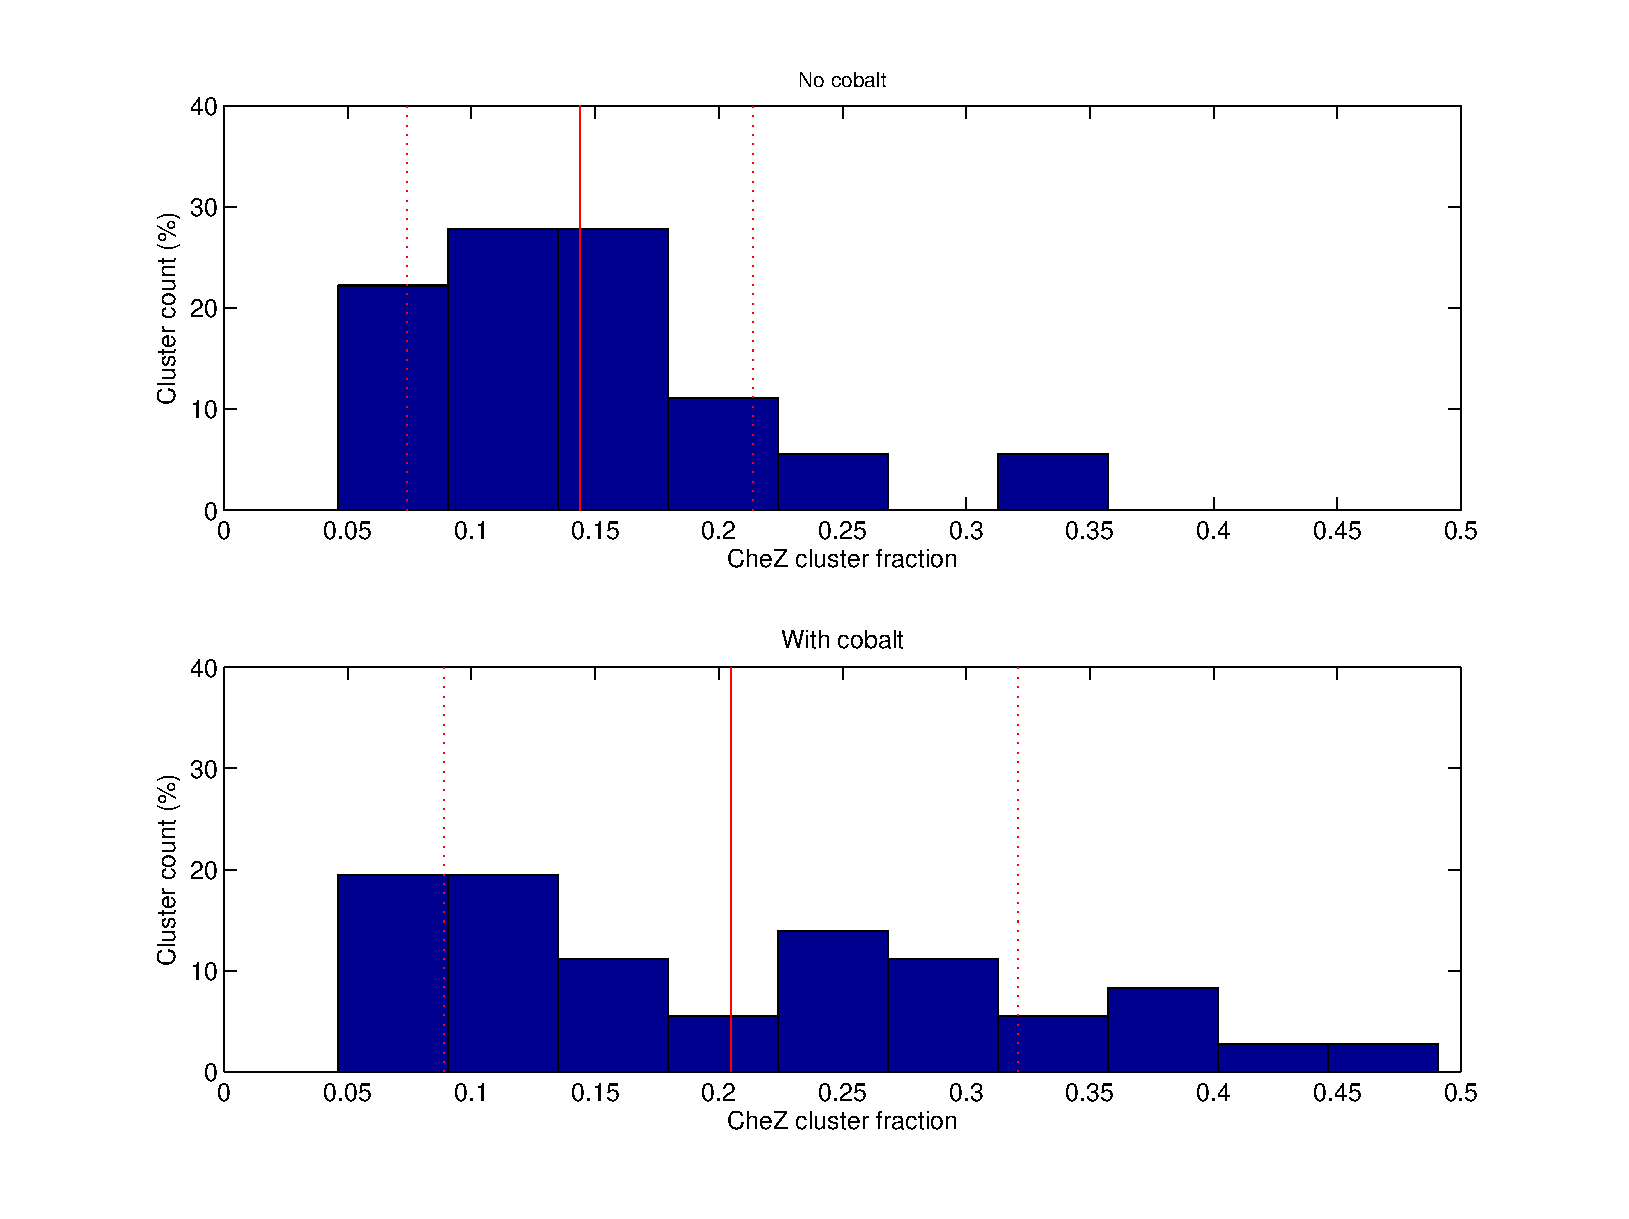
\includegraphics[scale=0.65, trim=0 30 0 310, clip=true]{\docroot results/figs/nikonb.eps}
	\label{fig:results:nikon:cobalt}
}
\caption[Image processing results on Nikon microscope]{Histograms of CheZ cluster fraction (fraction of CheZ protein in cell localised in the polar cluster). Solid red line marks mean average, dashed lines \(\pm\sigma\).}
\label{fig:results:nikon}
\end{center}
\end{figure}

\subsubsection{Confocal Microscopy}
\label{sec:results:cs:confocal}
These experiments were performed on a Zeiss confocal microscope, the use of which was kindly given to us by Alessandro Esposito at the Hutchison MRC. Ten images were taken each from a slide of cells prepared with and without cobalt.

\begin{figure}[h!]
\begin{center}
\subfloat[No cobalt, \(n=1222, \mu=0.185, \sigma=0.068\)]{
	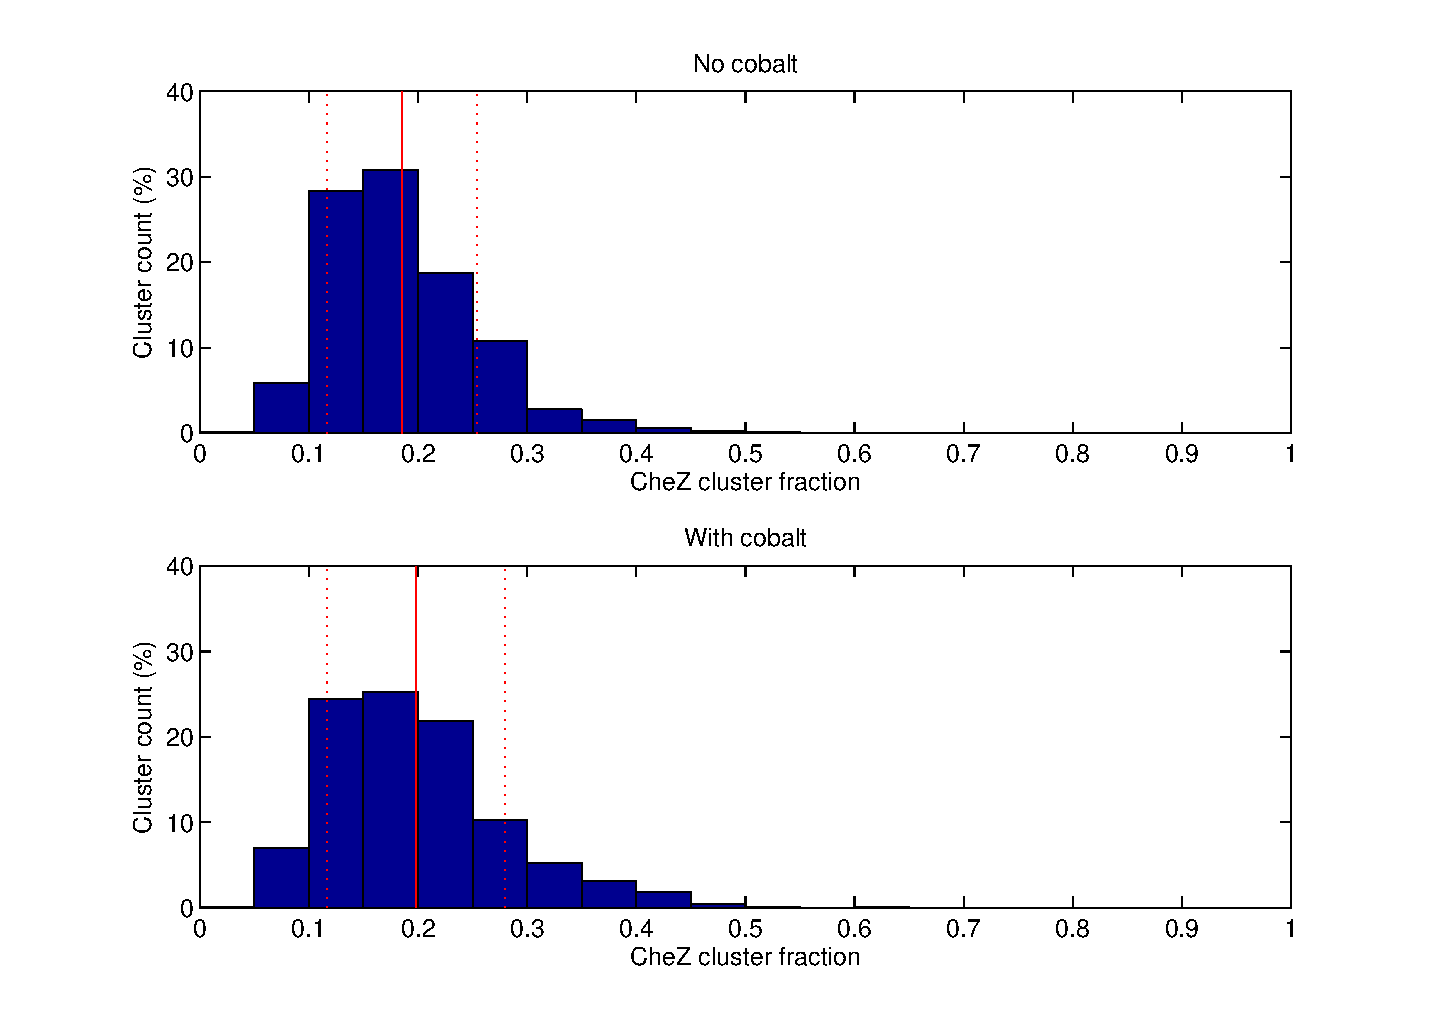
\includegraphics[scale=0.65, trim=0 250 0 30, clip=true]{\docroot results/figs/zeiss.eps}
	\label{fig:results:zeiss:nocobalt}
}\\
\subfloat[With cobalt, \(n=644, \mu=0.198, \sigma=0.082\)]{
	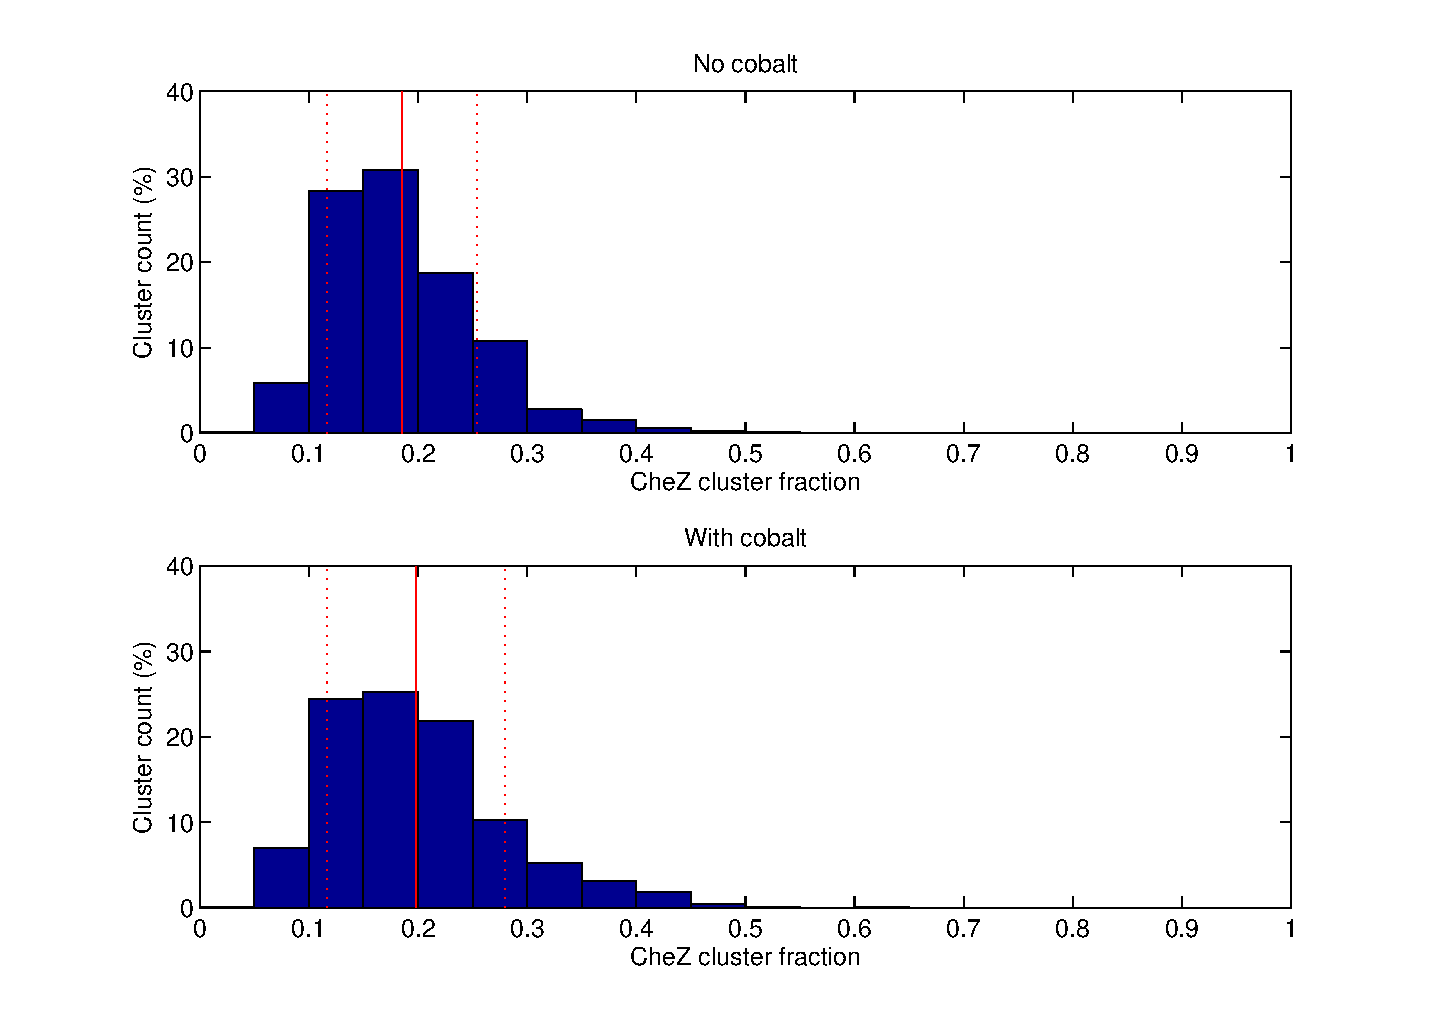
\includegraphics[scale=0.65, trim=0 20 0 260, clip=true]{\docroot results/figs/zeiss.eps}
	\label{fig:results:zeiss:cobalt}
}
\caption[Image processing results on Zeiss confocal microscope]{Histograms of CheZ cluster fraction (fraction of CheZ protein in cell localised in the polar cluster). Solid red line marks mean average, dashed lines \(\pm\sigma\). \(p\) value \(=0.0349\%\) using the Student's t-test.}
\label{fig:results:zeiss}
\end{center}
\end{figure}
\newpage

\subsection{PALM}

\begin{figure}[h!]
\begin{center}
\subfloat[Epifluorescent image]{
	\setlength\fboxsep{0pt}
	\setlength\fboxrule{1pt}
	\fbox{
		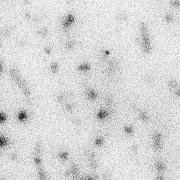
\includegraphics[height=.48\textwidth]{\docroot results/figs/PALMOriginal}
	}
	\label{fig:results:palm:original}
}
\subfloat[PALM reconstruction]{
	\fbox{
		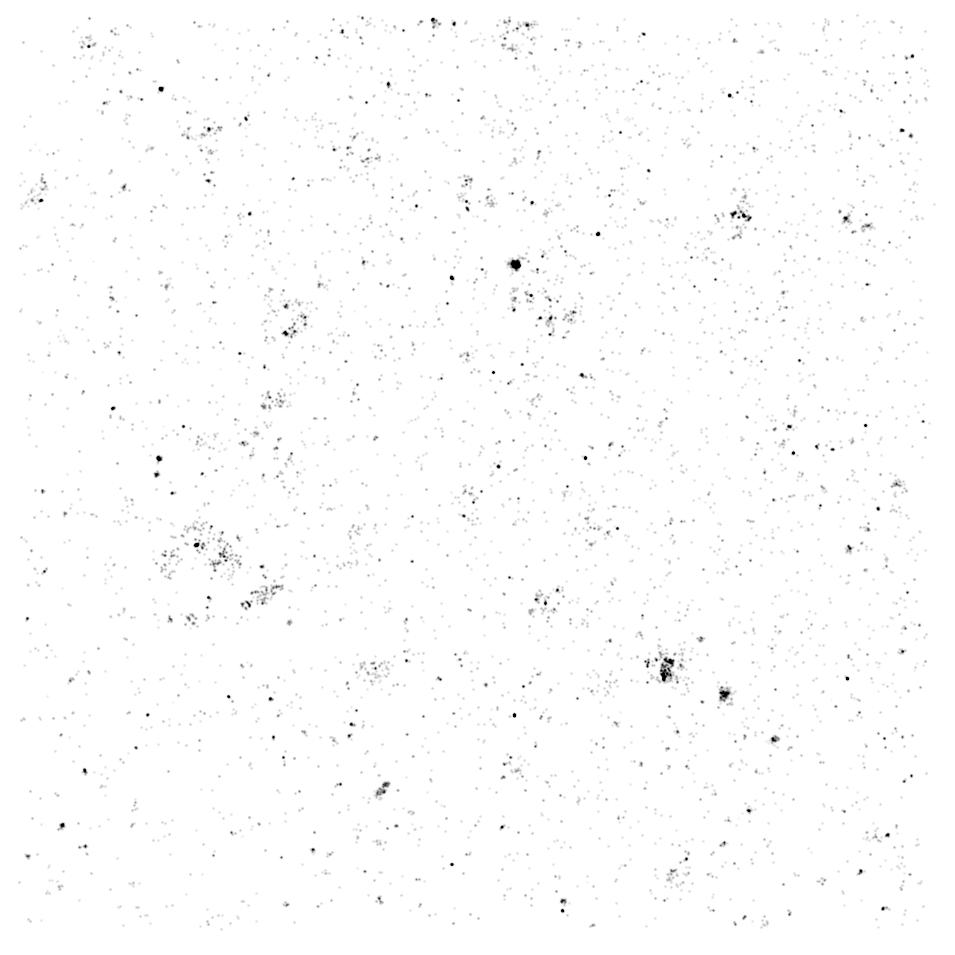
\includegraphics[height=.48\textwidth]{\docroot results/figs/PALMReconstruction}
	}
	\label{fig:results:palm:reconstruction}
}
\caption[PALM reconstruction]{PALM reconstruction of image. From 17990 frames in non-optimal media.}
\label{fig:results:palm}
\end{center}
\end{figure}
\newpage
\subsection{STED}
\begin{figure}[h!]
\begin{center}
\subfloat[Confocal microscopy]{
	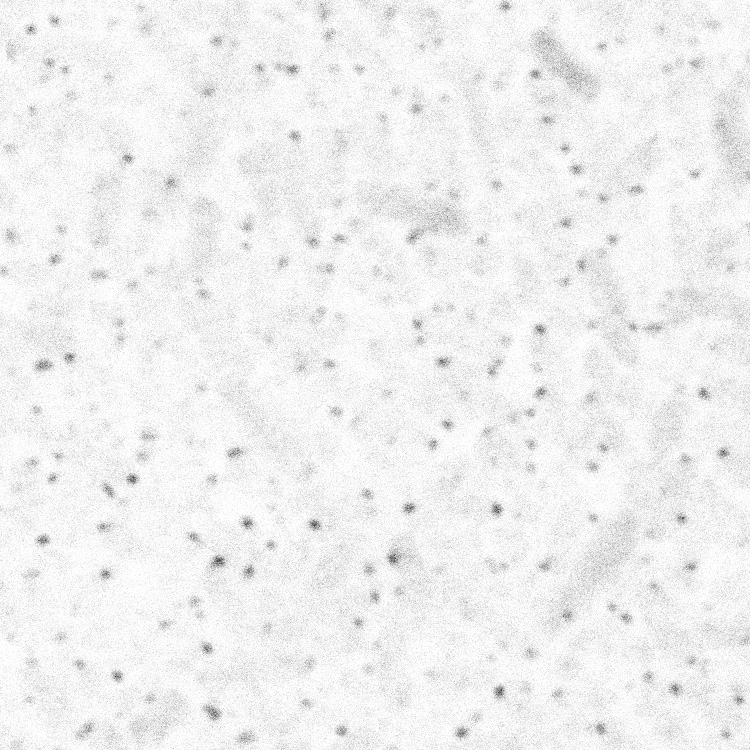
\includegraphics[width=0.45\textwidth]{\docroot results/figs/sted-con}
	\label{fig:results:sted:con}
}
\subfloat[STED Microscopy]{
	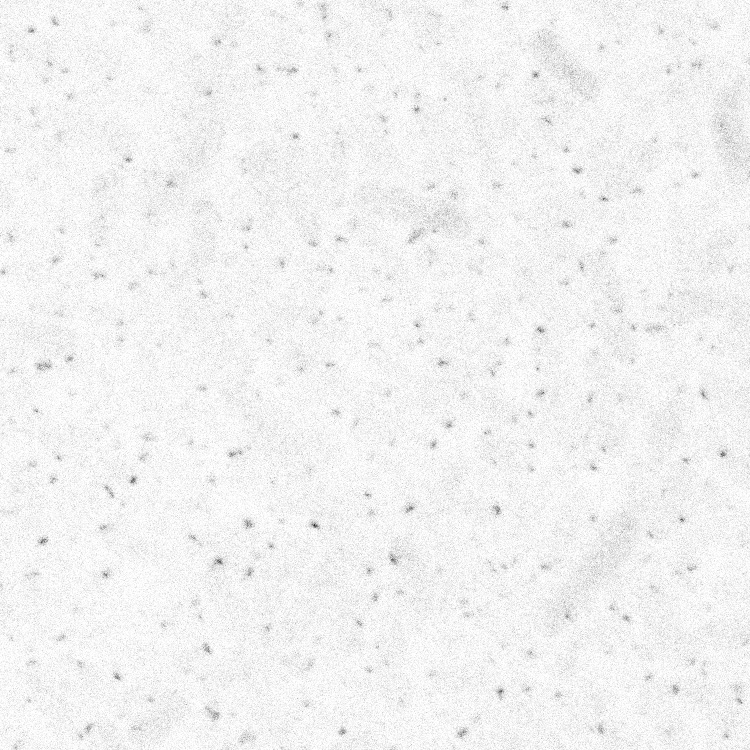
\includegraphics[width=0.45\textwidth]{\docroot results/figs/sted-sted}
	\label{fig:results:sted:sted}
}
\caption[STED microscopy]{STED Microscopy. Both images are of the same sample of KL1005 taken simultaneously. Colours inverted and contrasted adjusted identically, and cropped for clarity.}
\label{fig:results:sted}
\end{center}
\end{figure}
\newpage
\subsection{Microfluidics}

In order to obtain live imaging of the response to chemotactic chemicals, we must be able to replace the media in which the cells are contained with media of differing concentrations of attractant or repellent. Inspired by Howard Berg and Steven Block's work~\citep{berg84} we set out to create a microfluidics flow cell that would allow for precise exchange of media. Aladdin pumps from WPI-Europe were used due to their relatively well documented scripting capabilities and economy - precision was not as pressing concern as normally found in microfluidic applications. Two different microfluidic devices were required.

\begin{figure}[h!]
\begin{center}
\subfloat[Simple microfluidics device for step changes]{
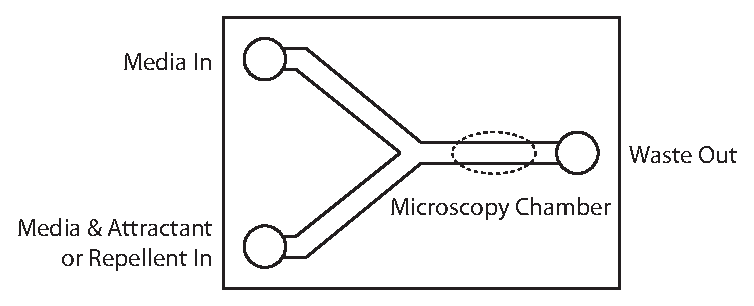
\includegraphics[scale=1]{\docroot results/figs/simplemicrofluidic.eps}
\label{fig:microfluidics:simple}
}\\
\subfloat[Complex microfluidics device for smooth mixing]{
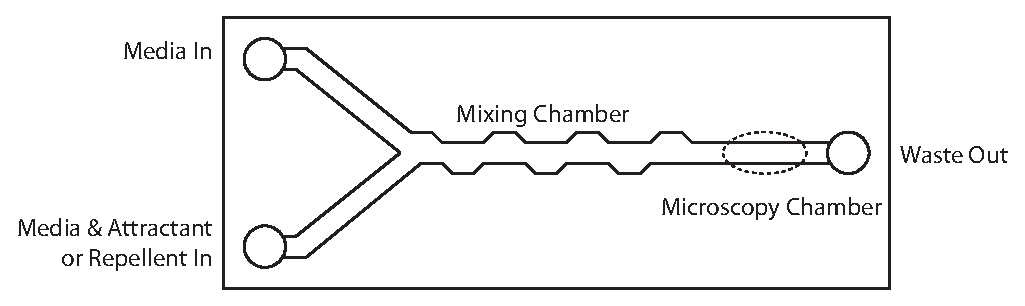
\includegraphics[scale=1]{\docroot results/figs/complexmicrofluidic.eps}
\label{fig:microfluidics:complex}
}
\caption[Microfluidics devices]{Schematics (not to scale) representative of the two types of microfluidics devices planned. The channels (parallel lines) are about \SI{1}{\milli\meter} wide and \SI{100}{\micro\meter} deep.}
\label{fig:microfluidics}
\end{center}
\end{figure}

The first, in Figure~\ref{fig:microfluidics:simple}, is a simple Y shaped splitter with only one syringe active at any time. One syringe would be filled with a plain media, and the other with media with attractant/repellent at a set concentration. This allows for rapid switching on and off of the attractant/repellent.

The second, in Figure~\ref{fig:microfluidics:complex}, is a more complex splitter to allow for thorough mixing of the two inputs. This takes the form of a zig-zag style channel between the two inputs and the chamber containing bacteria. Again, one syringe would be filled with a plain media, and the other with media with attractant/repellent at a set concentration. By varying the relative rates of the two pumps but keeping the total constant the concentration of attractant/repellent can be varied between zero and the aforementioned concentration. The drawback of this system is firstly the lag between changing pump speeds and observing a change in concentration in the bacterial chamber, and secondly the smoothing of a step change in concentration due to forward and backward diffusion of the attractant/repellent.

Flow cells were constructed from PDMS, bonded to \(\sim\)\SI{1}{\milli\meter} PDMS. We found that a deposit of live cells could be stuck to the inside surface of the flow cells by flushing them through with first poly-L-lysine, then blank media, then the cells, and finally blank media again.
\end{document}